\section{Phase II upgrade}
In the year 2023, the high luminosity LHC (HL-LHC) will begin operations of what is referred to as Phase II of the LHC. At that stage, the instantaneous luminosity will increase by a factor of 10 from its Run 1 design value, up to $\mathcal{L}\approx10^{35}$ cm$^{-2}$s$^{-1}$. A primary motivation for this transformation is to make it possible to study in great detail whatever phenomena may be discovered in the current phase of operation. This LHC upgrade will be accompanied by an upgrade in the hardware of the CMS detector, including improvements to various subsystems, and in some cases, the replacement of the old subsystems with new detectors. The tracker will likely be extended to cover the pseudorapidity range up to $|\eta|<4$, the muon system will likewise be extended into the forward region, the level 1 trigger system will be modified so that it considers information from the tracker in addition to the calorimeters and muon system, and the ECAL and HCAL endcaps will be replaced by more sophisticated detectors. 

Work has been carried out in preparation for the last item in this list, the calorimeter endcap upgrade. This section describes a portion of this work that I carried out. Some of the results were shown at the 2014 CMS upgrade Jamboree, and were included as part of the information that informed the decision of the down-select, in which one endcap design was selected for construction. 

\subsection{Calorimeter research and development}

Two options were considered for the set of detectors that will replace the CMS endcaps during the Phase II upgrade \cite{Bilki:2015rla}: a sampling ``shashlik'' calorimeter, and a high granularity calorimeter (HGCAL). Ultimately, the HGCAL design was chosen for construction. The shashlik calorimeter, in design, is composed of towers 114 mm in length with square cross sections of $14\times14$ mm. Each tower (Figure \ref{fig:shashtower})
\begin{figure}[h]\centering
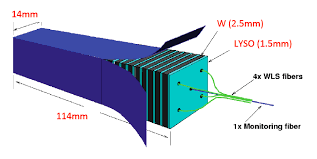
\includegraphics[width=0.6\linewidth]{figures/CMS/Upgrade/ShashlikTower.png}\\
\caption{A shashlik calorimeter tower. }
\label{fig:shashtower}
\end{figure}
is composed of 28 layers of Tungsten alternating with 29 layers of LYSO, where LYSO (LuYSiO$_5$(Ce)) is a high density (7.1 g/cm$^3$) scintillating material largely developed for use in particle detectors by Caltech \cite{Chen:2007bb}. The HGCAL is a sampling calorimeter that will be built from alternating lead and copper sampling layers, with signal readout from silicon photosensors. The HGCAL design is notable for its ability to provide longitudinal as well as lateral information about the distribution of energy deposited by high-energy particles.

In April-May of 2014 and July-August, 2014, test beam experiments were held at Fermilab at the M-Test facility~\cite{Fermi:T1041} to study and characterize a prototype module of the shashlik calorimeter (Figure \ref{fig:shashscatter} illustrates the prototype structure). 
\begin{figure}[h]\centering
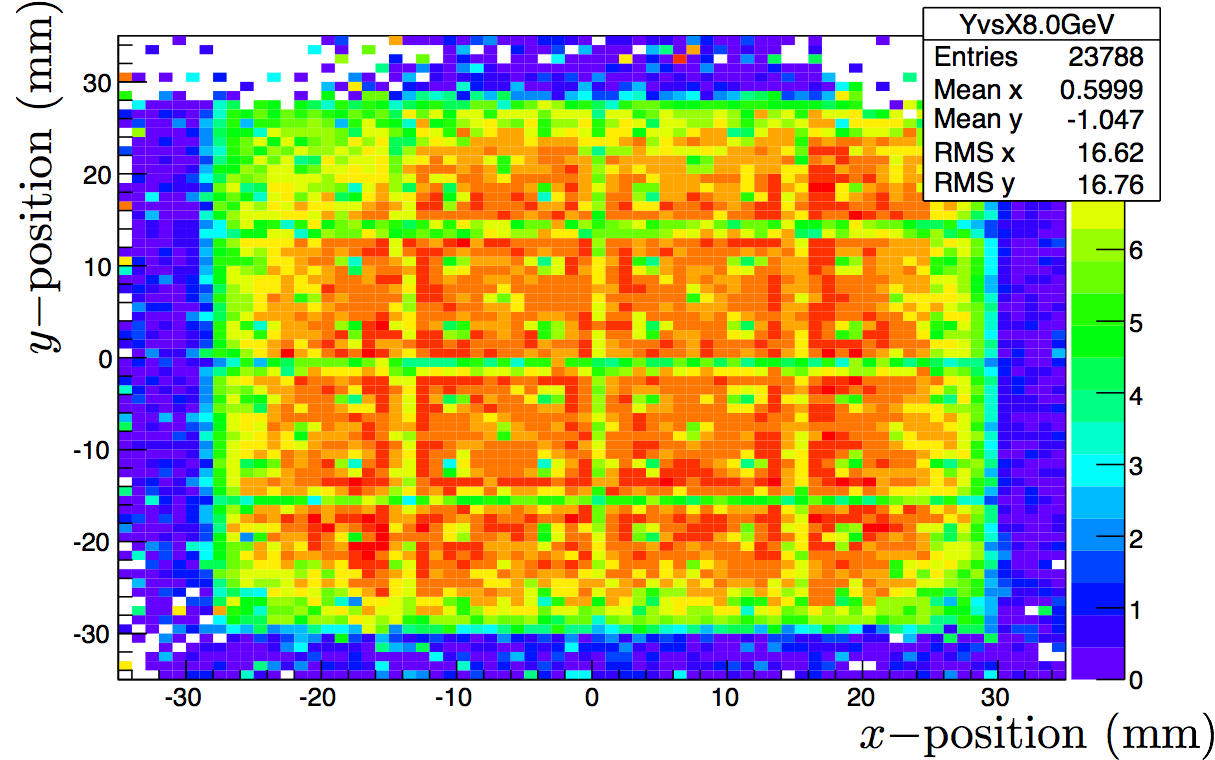
\includegraphics[width=0.6\linewidth]{figures/CMS/Upgrade/TopoMap.png}\\
\caption{A scatter plot of the accumulated track positions weighted by the in-time energy deposited in the shashlik tower, for a set of muon runs recorded in July, 2014. The $4\times4$ tower array structure, the gaps between towers, and the holes bored for the WLS fibers can be seen as green features.}
\label{fig:shashscatter}
\end{figure}
The testbeam facility provided access to beams of particles with an energy per particle ranging from 1 to 120 GeV. Several characteristics of the beam could be chosen in real time, such as the species of particles populating the beam, as well as the energy per particle.  The facility also provided the use of two wire chambers, which were used to determine the time and position of incident particles.The shashlik prototype consisted of a $4\times4$ array of towers, and each tower (Figure \ref{fig:shashtower})
\ref{fig:shashtower})
was read out by four wavelength-shifting (WLS) fibers fed longitudinally through the towers and connected to silicon photomultiplier sensors (SiPMs). 

While working help set up and manage the testbeams, I authored an interactive event display that was used to view data as it was being collected. The event display is a flexible, python-based program with a graphical user interface (GUI) that can be be used to view both live as well as stored data. The GUI is largely based on the TEve class of the Root software package \cite{Brun:1997pa}, which makes use of a slots and signals framework to enable communication between objects defined in the program. Signals carry information related to one or several user-defined objects, can be produced as a result of various actions taken by the user or from the data stream, while slots are a class of objects that are capable of receiving this information and initiating changes to their associated user-defined objects. For a concrete example, after processing the tracking information for a given event, the program produces a signal that is received by the module that projects a 3-dimensional event view, which is updated to display a set of tracks.

The event display contains several view panels, including 
\begin{itemize}
\item a heat map (color plot) of the maximum analog-to-digital count (ADC) recorded by each channel during an event in real space, as shown in Fig. \ref{fig:HeatMaps} (top);
\item a display of the readout and $\chi^2$ of the samples by channel, and a display of the pedestal noise, as shown in Fig. \ref{fig:HeatMaps}, (bottom);
\item a display of the pedestal noise by channel, where the pedestal is the expected number of ADC counts in the absence of any signal, as shown in Fig. \ref{fig:NoiseAndWires};
\item a view of the in time hits in the wire chambers, where ``in time'' refers to the criterion that the recorded time of the signal be consistent with the time of the recorded energy deposited in the calorimeter, as shown in Fig. \ref{fig:NoiseAndWires}, and
\item a 3-dimensional view of of the hits, tracks, wire chambers, and the shashlik calorimeter with color corresponding to the estimated energy deposited in each tower, as shown in Fig. \ref{fig:Shashlik3d}.
\end{itemize}
\begin{figure}[h]\centering
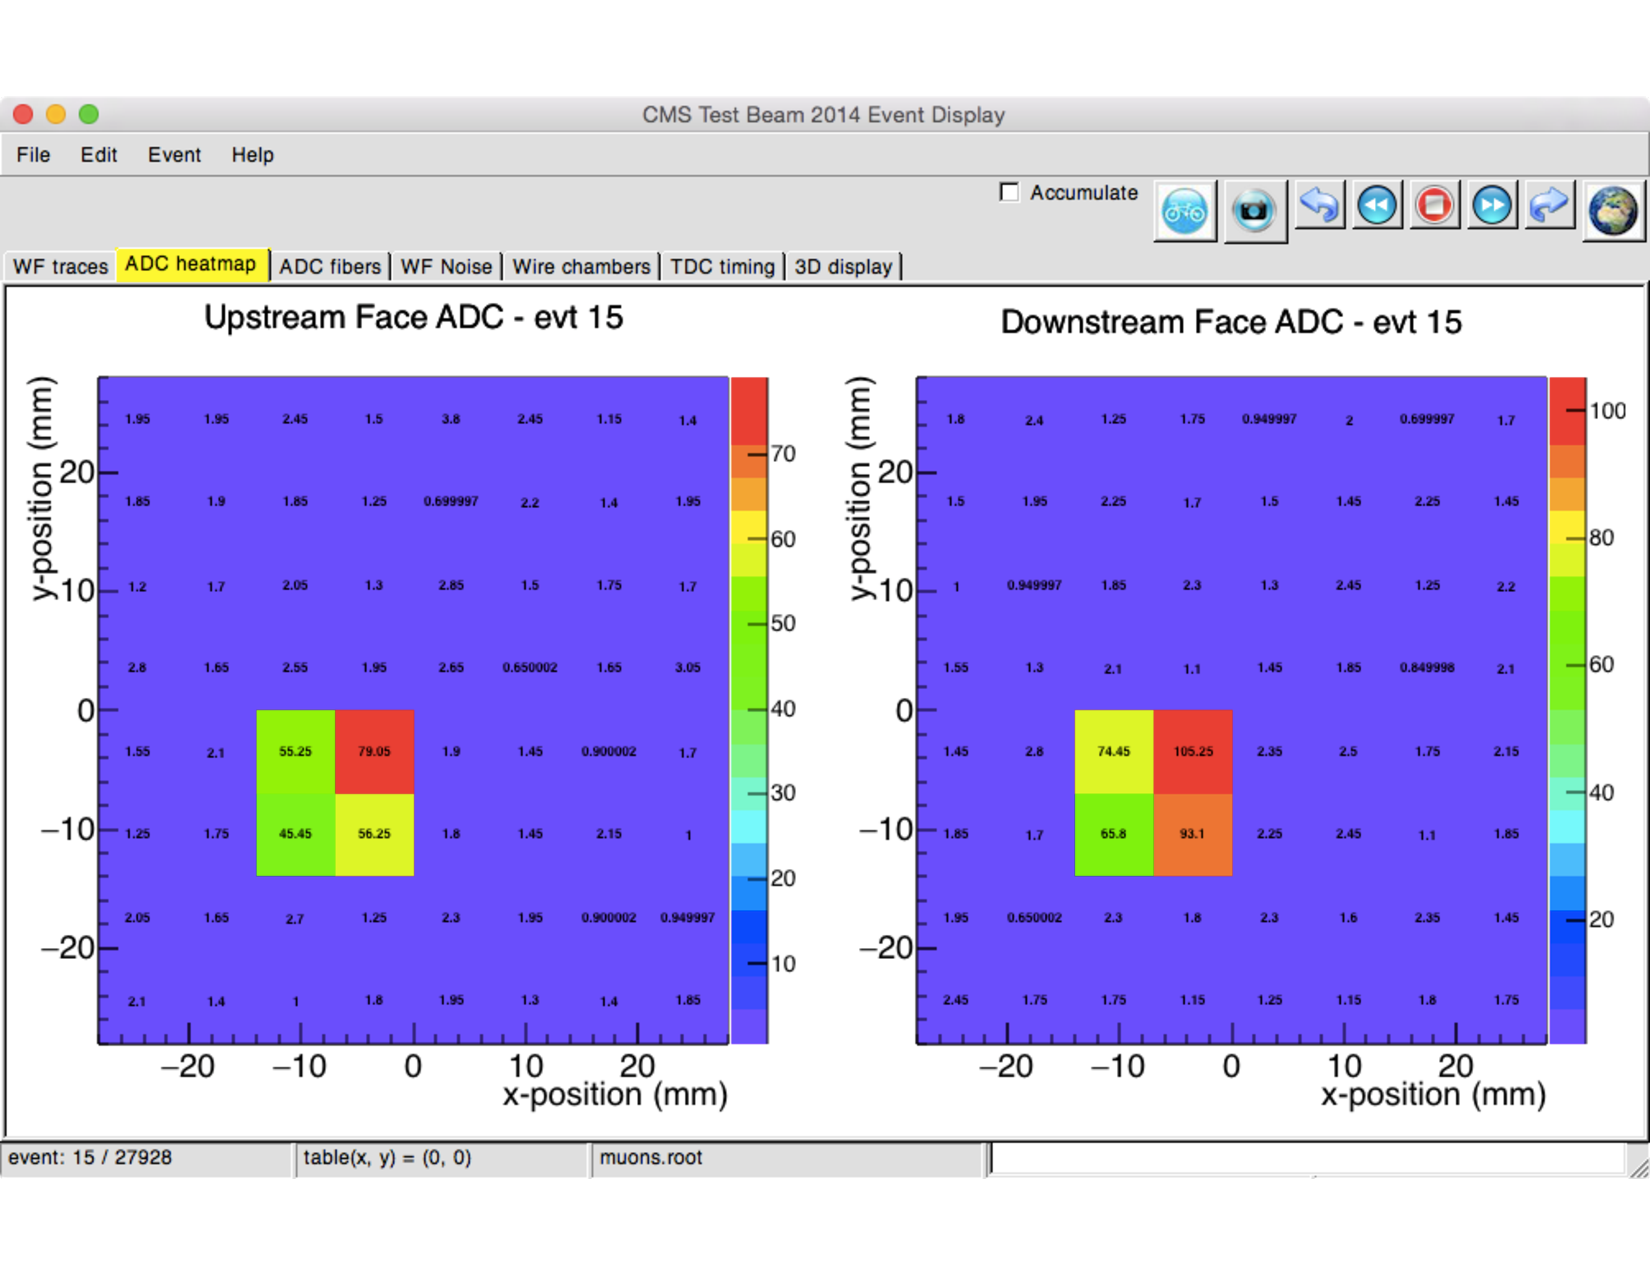
\includegraphics[width=0.85\linewidth]{figures/CMS/Upgrade/MuonHeatMap.pdf}\\
\vspace{-1cm}
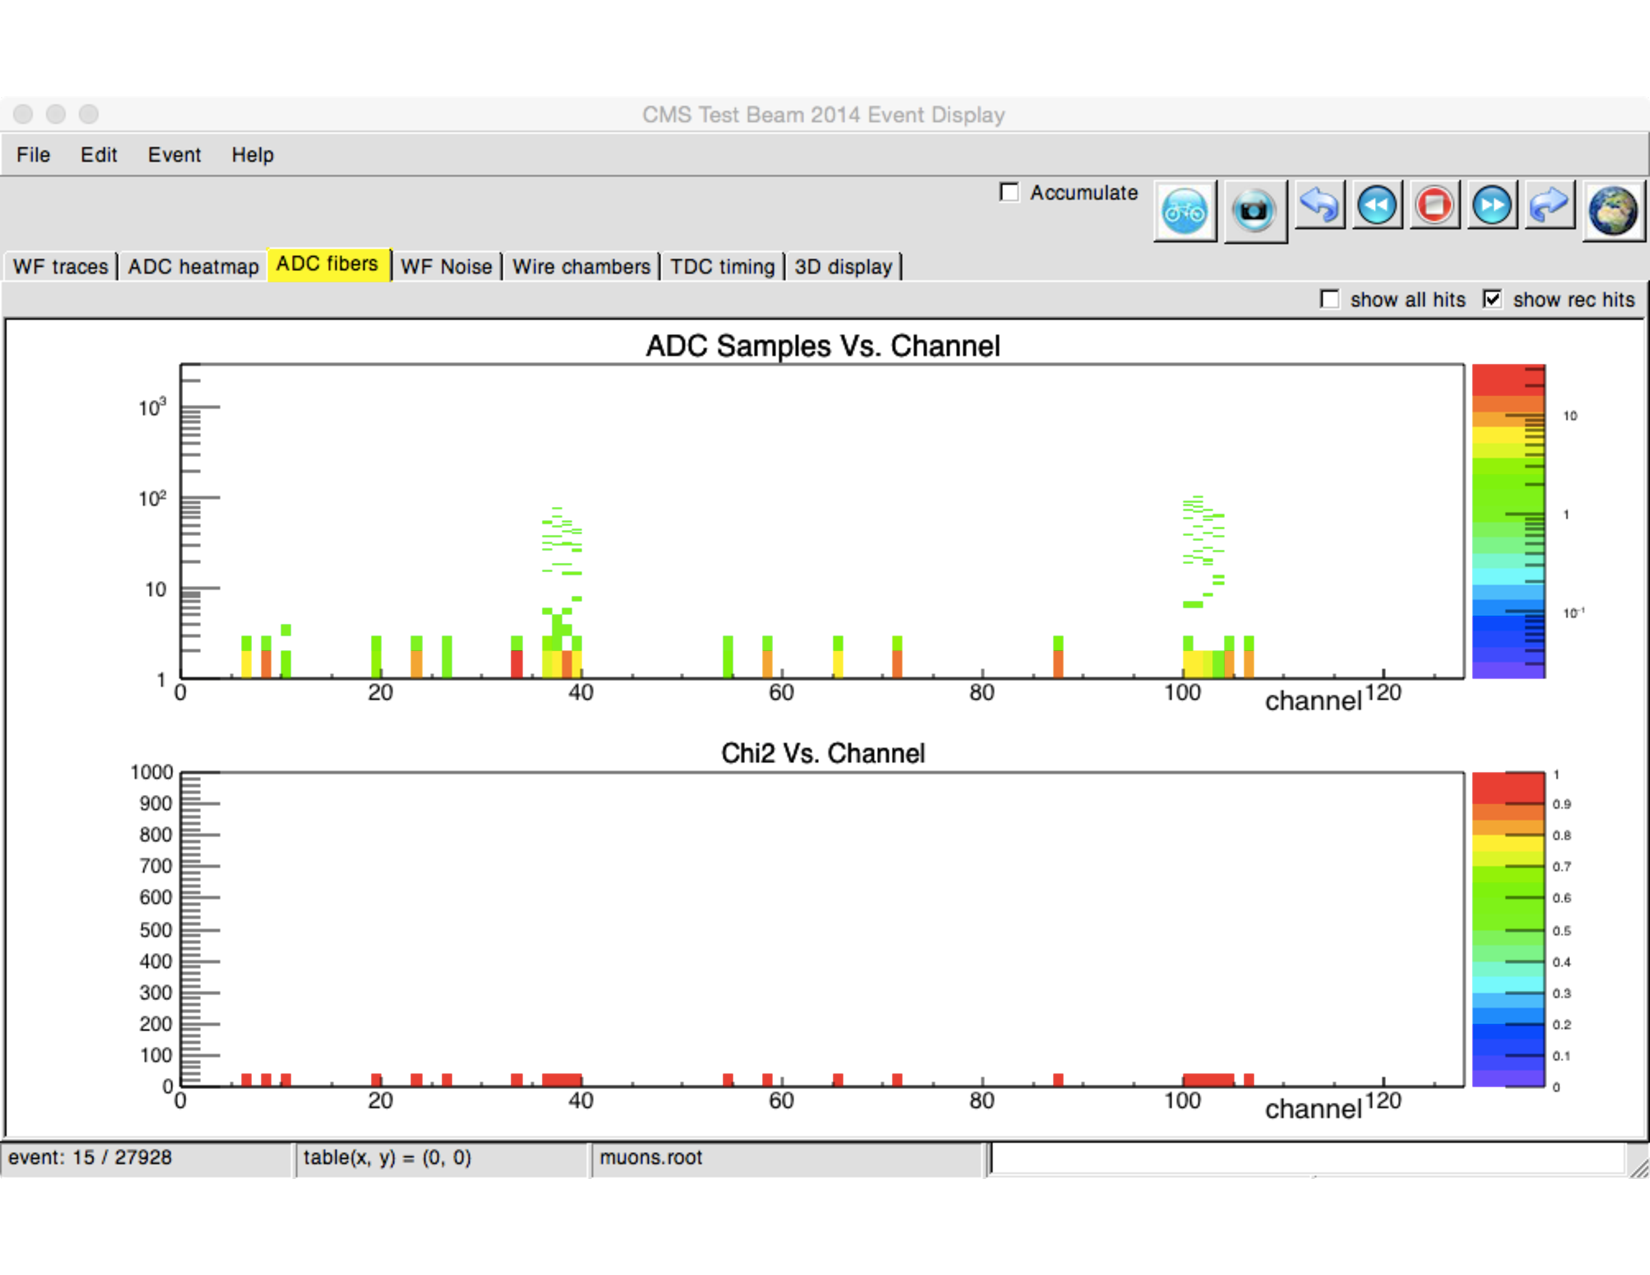
\includegraphics[width=0.85\linewidth]{figures/CMS/Upgrade/HealthyPulses.pdf}
\caption{Top: heat maps of the ADC counts recorded at the upstream and downstream faces of the shashlik module. Bottom: Diagnostic displays of channel-by-channel information from the shashlik module. The "Chi2 Vs. Channel" display is effective at revealing noisy channels, that is, channels with a large ADC count generated by electronic noise rather than a genuine particle signal.}
\label{fig:HeatMaps}
\end{figure}
\begin{figure}[h]\centering
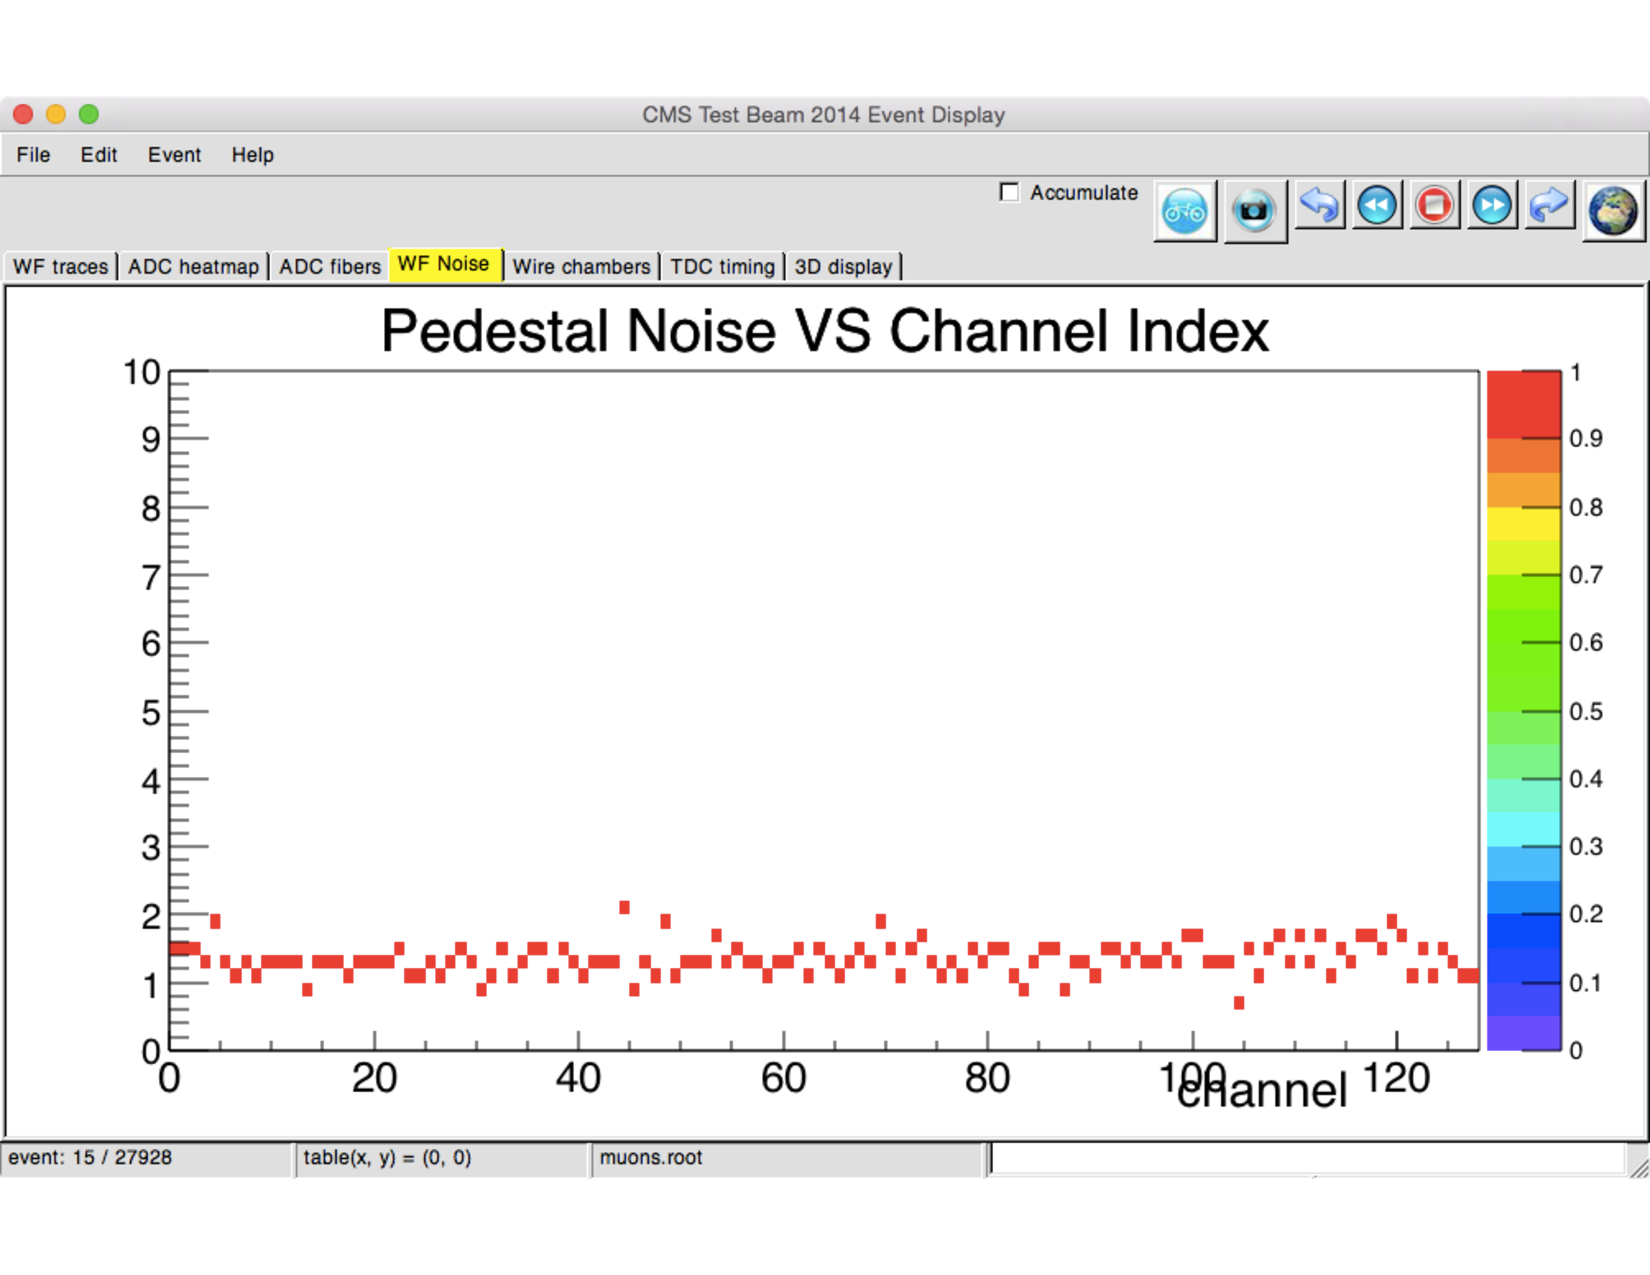
\includegraphics[width=0.8\linewidth]{figures/CMS/Upgrade/PedestalNoise.pdf}\\
\vspace{-1cm}
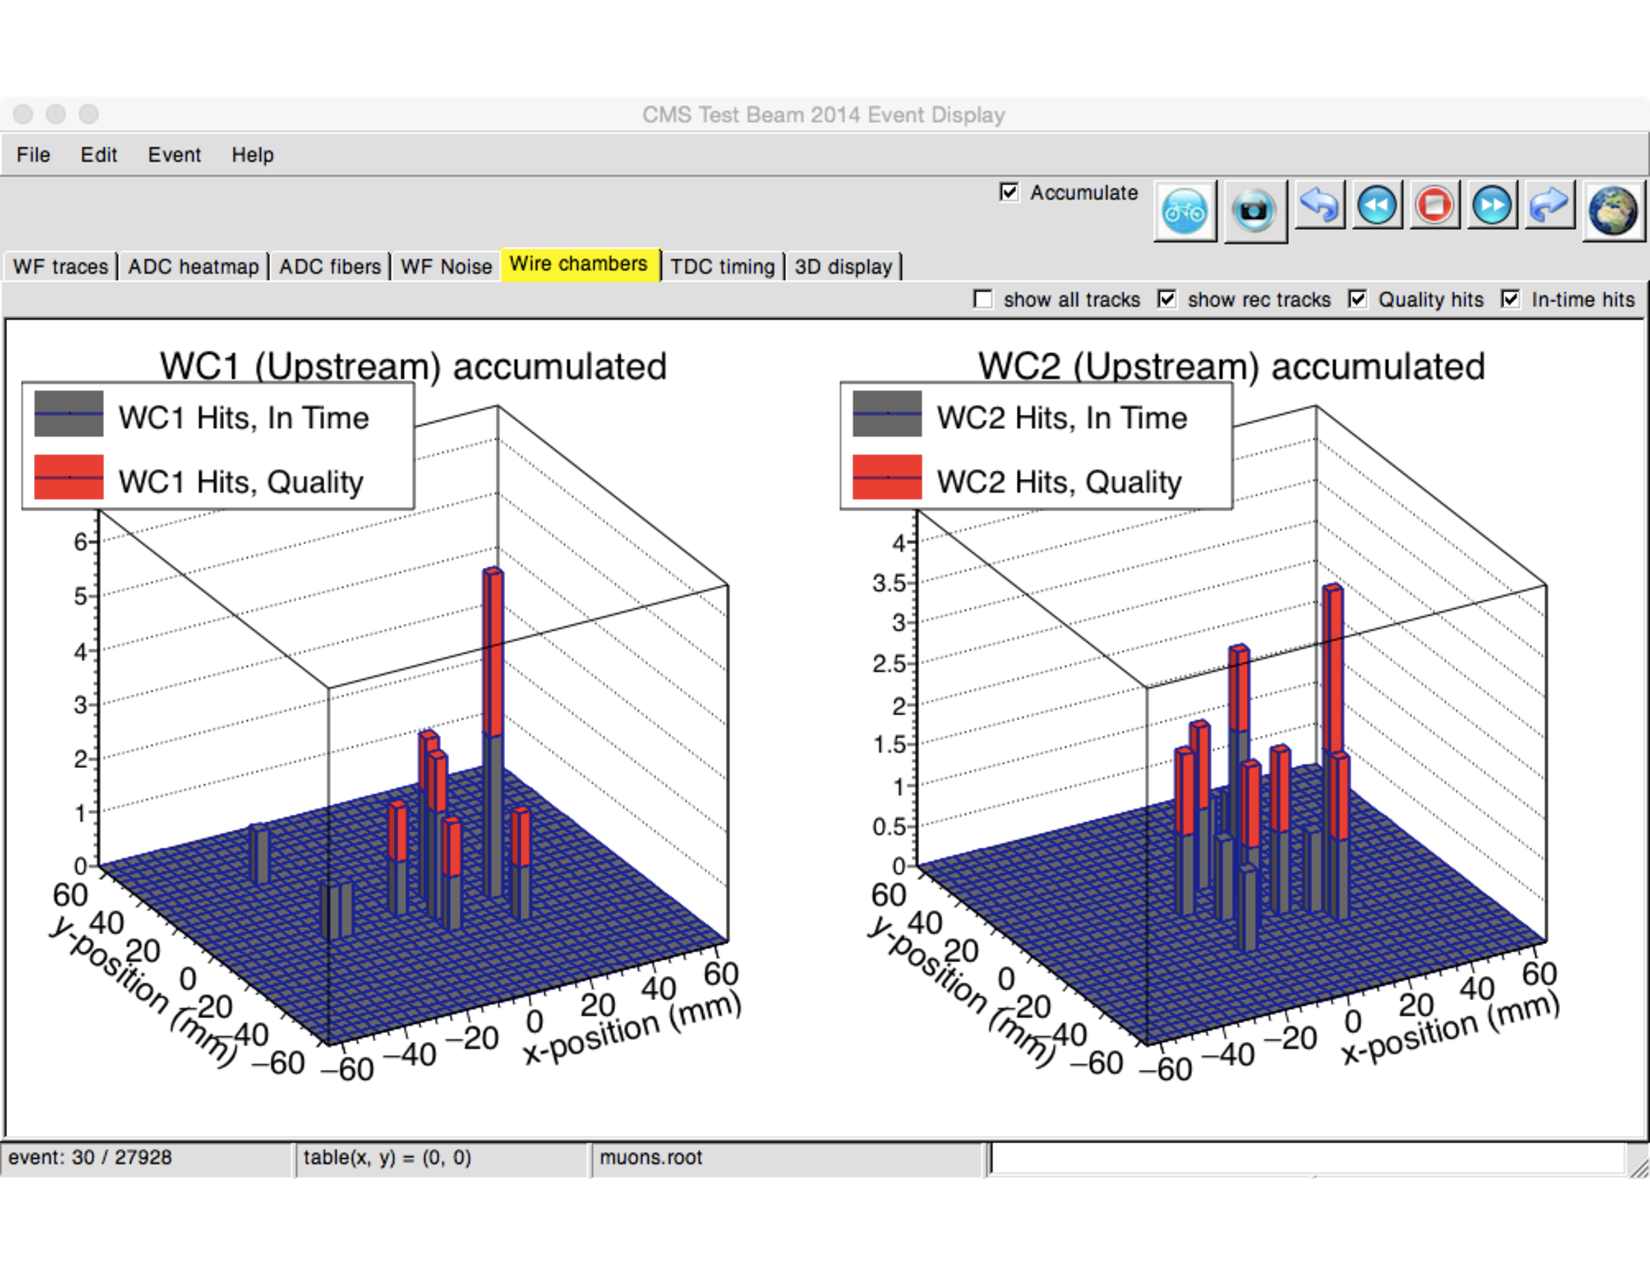
\includegraphics[width=0.8\linewidth]{figures/CMS/Upgrade/WireChambers.pdf}
\caption{Top: The pedestal noise by channel. Bottom: A scatter plot of the positions of accumulated hits and tracks recorded by the wire chambers; quality hits are colored red, and refer to hits consistent with a particle track.}
\label{fig:NoiseAndWires}
\end{figure}
\begin{figure}[h]\centering
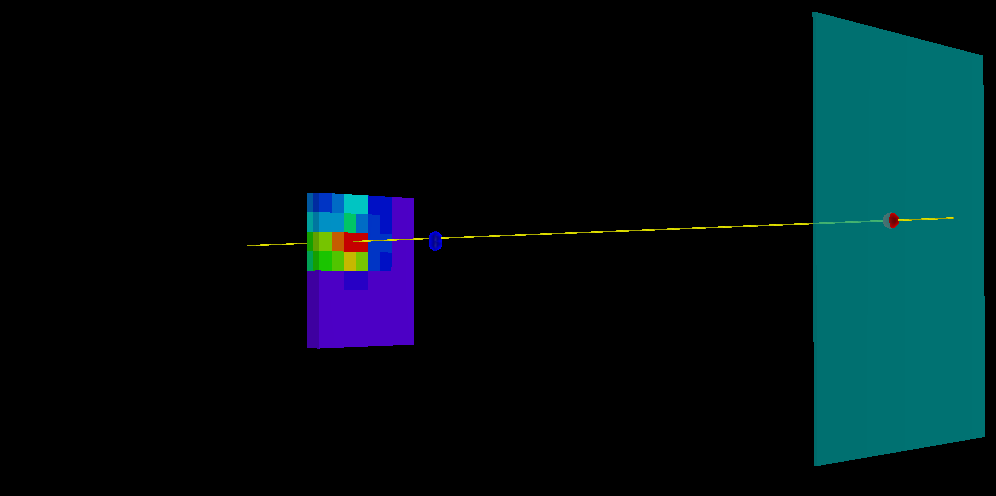
\includegraphics[width=0.8\linewidth]{figures/CMS/Upgrade/3D_50.png}\\
\vspace{0.8cm}
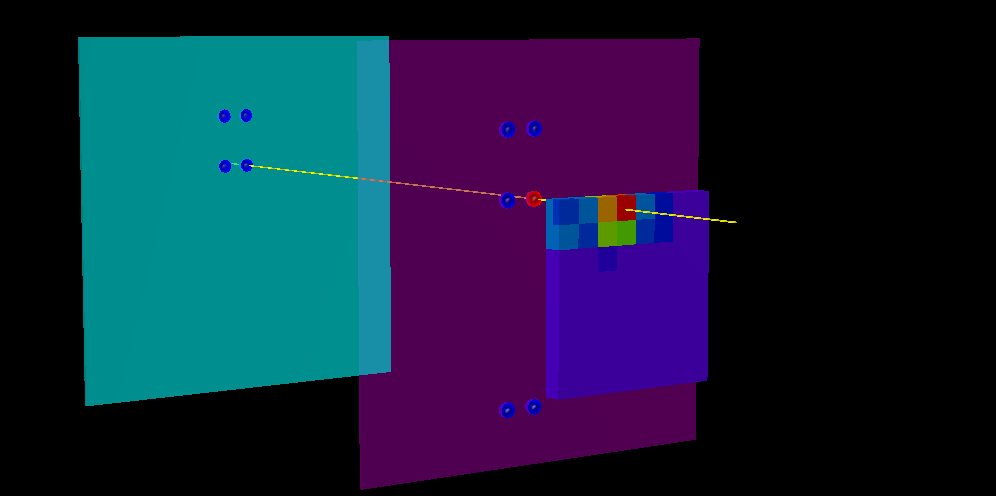
\includegraphics[width=0.8\linewidth]{figures/CMS/Upgrade/3D_14.png}
\vspace{0.8cm}
\caption{Three-dimensional views of reconstructed tracks and calorimetric energy deposits in events containing a 120 GeV proton. The view can be rotated by the user, allowing different viewing perspectives of the event, as illustrated in the top and bottom figures.}
\label{fig:Shashlik3d}
\end{figure}
\noindent
The event display has since been adopted for use at testbeam experiments dedicated to studying the HGCAL, where a prototype of the future calorimeter is being characterized. The software for the event display can be obtained at the url in Ref.~\cite{bib:EventDisplay}. 

\subsubsection{Jet/\MET analysis}
After testbeam operations, I and my colleague Arka Santra performed analysis of the data collected, as well as of simulated events. The energy resolution of jets in the CMS endcaps for various phases of the CMS detector are shown in Fig. \ref{fig:ShashlikResolution}.
\begin{figure}[h]
\centering
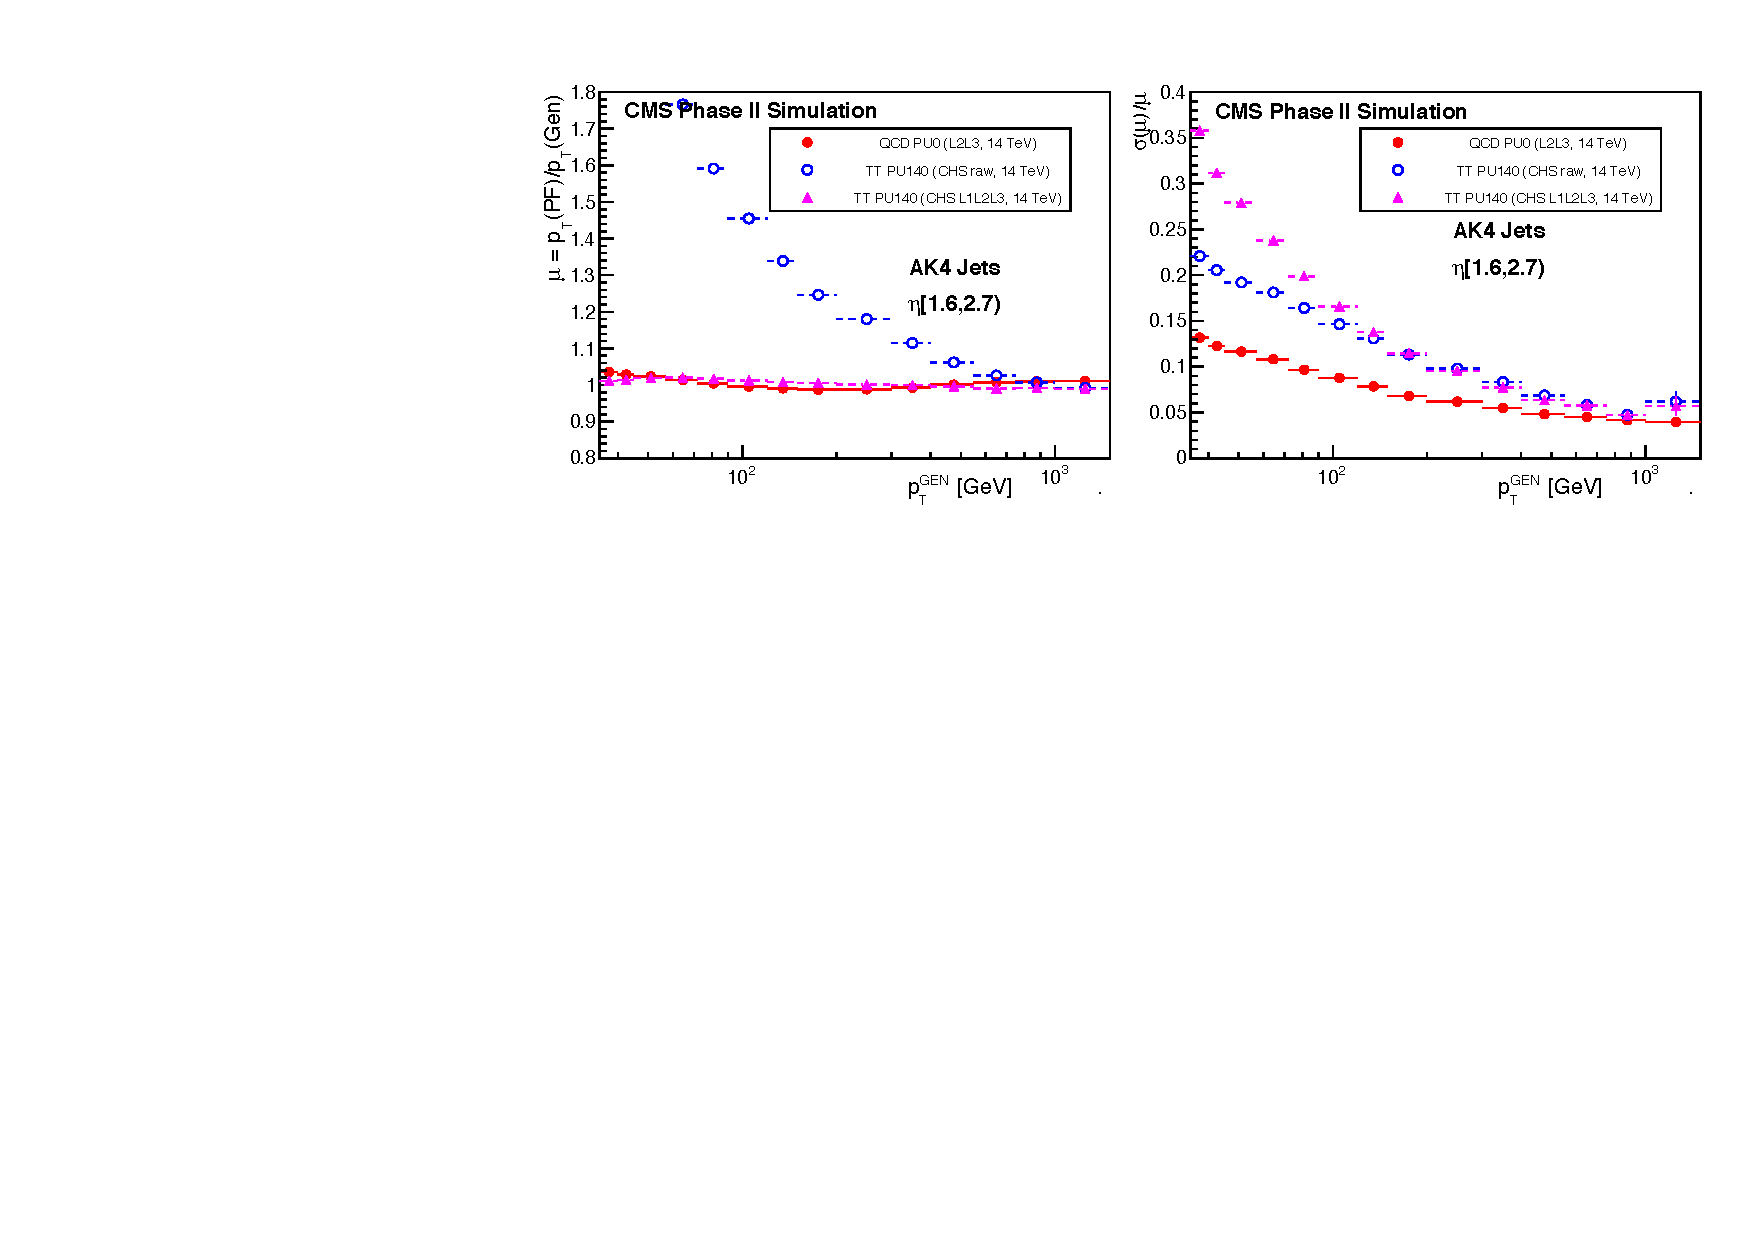
\includegraphics[width=0.9\linewidth]{figures/CMS/Upgrade/ChsJetPerformanceEndcapTT.pdf}
\caption{The jet response (left) and energy resolution (right) in the shashlik endcap as a function of simulated jet $p_T$ in a sample of simulated $t\bar{t}$ events. The red distributions correspond to the scenario without pile-up, and pink to that with pile-up of 140 (an average of 140 collisions per bunch crossing), which is the expected amount of pile-up during the post-Phase II LHC operations. }
\label{fig:ShashlikResolution}
\end{figure}
At large $p_T$, the energy resolution in PU 140 events is seen to drop below 10\%, indicating an excellent level of performance that surpasses that described in Ref.~\cite{Bilki:2015rla}.

\FloatBarrier




